\documentclass[tikz,border=2pt]{standalone}
\usepackage{amsmath}
\usepackage{pgfplots}
\pgfplotsset{compat=1.18}
\usetikzlibrary{arrows.meta}
\begin{document}
% Theorem 2.1a/b, Example 1: V1=Cl(B(0;1)), V2=Cl(B((4,3);2)), a=(4,3); max over V1 of a^T x is 5, min over V2 is 15,
% so {4x1+3x2=b} separates for every b in [5,15] (shaded strip): b=5 touches V1 at (0.8,0.6), b=15 touches V2 at (2.4,1.8),
% b=10 meets neither set.
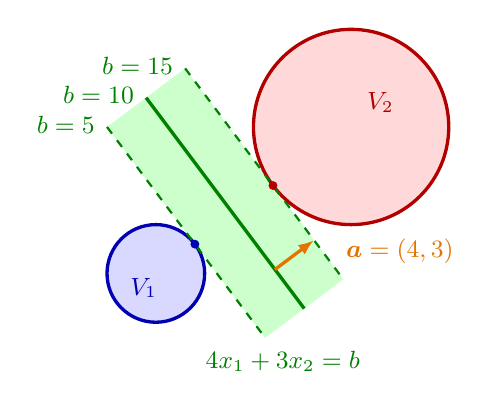
\begin{tikzpicture}[font=\small, >={Latex[length=2mm]}, x=0.62cm, y=0.62cm]
  % strip of separating hyperplanes 5 <= 4x1+3x2 <= 15
  \fill[green!20] (-1,3) -- (0.6,4.2) -- (3.84,-0.12) -- (2.24,-1.32) -- cycle;
  % the two discs
  \fill[blue!15] (0,0) circle (1);
  \draw[blue!70!black, very thick] (0,0) circle (1);
  \fill[red!15] (4,3) circle (2);
  \draw[red!70!black, very thick] (4,3) circle (2);
  \node[blue!70!black] at (-0.25,-0.3) {$V_1$};
  \node[red!70!black] at (4.6,3.5) {$V_2$};
  % hyperplanes 4x1+3x2=b for b=5,10,15
  \draw[green!50!black, thick, dashed] (-1,3) -- (2.24,-1.32);
  \draw[green!50!black, very thick] (-0.2,3.6) -- (3.04,-0.72);
  \draw[green!50!black, thick, dashed] (0.6,4.2) -- (3.84,-0.12);
  \node[green!50!black, anchor=east] at (-1.05,3.05) {$b=5$};
  \node[green!50!black, anchor=east] at (-0.25,3.65) {$b=10$};
  \node[green!50!black, anchor=east] at (0.55,4.25) {$b=15$};
  \node[green!50!black, anchor=north] at (2.6,-1.4) {$4x_1+3x_2=b$};
  % touching points
  \fill[blue!70!black] (0.8,0.6) circle (1.6pt);
  \fill[red!70!black] (2.4,1.8) circle (1.6pt);
  % normal a=(4,3)
  \draw[orange!90!black, very thick, ->] (2.44,0.08) -- (3.24,0.68);
  \node[orange!90!black, anchor=west] at (3.7,0.45) {$\boldsymbol{a}=(4,3)$};
\end{tikzpicture}
\end{document}
